%% (Master) Thesis template
% Template version used: v1.4
%
% Largely adapted from Adrian Nievergelt's template for the ADPS
% (lecture notes) project.


%% We use the memoir class because it offers a many easy to use features.
\documentclass[11pt,a4paper,titlepage]{memoir}

%% Packages
%% ========

%% LaTeX Font encoding -- DO NOT CHANGE
\usepackage[OT1]{fontenc}

%% Babel provides support for languages.  'english' uses British
%% English hyphenation and text snippets like "Figure" and
%% "Theorem". Use the option 'ngerman' if your document is in German.
%% Use 'american' for American English.  Note that if you change this,
%% the next LaTeX run may show spurious errors.  Simply run it again.
%% If they persist, remove the .aux file and try again.
\usepackage[english]{babel}

%% Input encoding 'utf8'. In some cases you might need 'utf8x' for
%% extra symbols. Not all editors, especially on Windows, are UTF-8
%% capable, so you may want to use 'latin1' instead.
\usepackage[utf8]{inputenc}

%% This changes default fonts for both text and math mode to use Herman Zapfs
%% excellent Palatino font.  Do not change this.
\usepackage[sc]{mathpazo}

%% The AMS-LaTeX extensions for mathematical typesetting.  Do not
%% remove.
\usepackage{amsmath,amssymb,amsfonts,mathrsfs}

%% NTheorem is a reimplementation of the AMS Theorem package. This
%% will allow us to typeset theorems like examples, proofs and
%% similar.  Do not remove.
%% NOTE: Must be loaded AFTER amsmath, or the \qed placement will
%% break
\usepackage[amsmath,thmmarks]{ntheorem}

%% LaTeX' own graphics handling
\usepackage{graphicx}

%% We unfortunately need this for the Rules chapter.  Remove it
%% afterwards; or at least NEVER use its underlining features.
\usepackage{soul}

%% This allows you to add .pdf files. It is used to add the
%% declaration of originality.
\usepackage{pdfpages}

\usepackage{biblatex}
\addbibresource{refs.bib}
%\bibliographystyle{plain}
\bibliography{refs}

%% Some more packages that you may want to use.  Have a look at the
%% file, and consult the package docs for each.
%% See the TeXed file for more explanations

%% [OPT] Multi-rowed cells in tabulars
%\usepackage{multirow}

%% [REC] Intelligent cross reference package. This allows for nice
%% combined references that include the reference and a hint to where
%% to look for it.
\usepackage{varioref}

%% [OPT] Easily changeable quotes with \enquote{Text}
%\usepackage[german=swiss]{csquotes}

%% [REC] Format dates and time depending on locale
\usepackage{datetime}

%% [OPT] Provides a \cancel{} command to stroke through mathematics.
%\usepackage{cancel}

%% [NEED] This allows for additional typesetting tools in mathmode.
%% See its excellent documentation.
\usepackage{mathtools}

%% [ADV] Conditional commands
%\usepackage{ifthen}

%% [OPT] Manual large braces or other delimiters.
%\usepackage{bigdelim, bigstrut}

%% [REC] Alternate vector arrows. Use the command \vv{} to get scaled
%% vector arrows.
\usepackage[h]{esvect}

%% [NEED] Some extensions to tabulars and array environments.
\usepackage{array}

%% [OPT] Postscript support via pstricks graphics package. Very
%% diverse applications.
%\usepackage{pstricks,pst-all}

%% [?] This seems to allow us to define some additional counters.
%\usepackage{etex}

%% [ADV] XY-Pic to typeset some matrix-style graphics
%\usepackage[all]{xy}

%% [OPT] This is needed to generate an index at the end of the
%% document.
%\usepackage{makeidx}

%% [OPT] Fancy package for source code listings.  The template text
%% needs it for some LaTeX snippets; remove/adapt the \lstset when you
%% remove the template content.
\usepackage{listings}
\lstset{language=TeX,basicstyle={\normalfont\ttfamily}}

%% [REC] Fancy character protrusion.  Must be loaded after all fonts.
\usepackage[activate]{pdfcprot}

%% [REC] Nicer tables.  Read the excellent documentation.
\usepackage{booktabs}

%Used To handle acronyms
\usepackage[printonlyused, footnote ]{acronym}


%% Our layout configuration.  DO NOT CHANGE.
%% Memoir layout setup

%% NOTE: You are strongly advised not to change any of them unless you
%% know what you are doing.  These settings strongly interact in the
%% final look of the document.

% Dependencies
\usepackage{ETHlogo}

% Turn extra space before chapter headings off.
\setlength{\beforechapskip}{0pt}

\nonzeroparskip
\parindent=0pt
\defaultlists

% Chapter style redefinition
\makeatletter

\if@twoside
  \pagestyle{Ruled}
  \copypagestyle{chapter}{Ruled}
\else
  \pagestyle{ruled}
  \copypagestyle{chapter}{ruled}
\fi
\makeoddhead{chapter}{}{}{}
\makeevenhead{chapter}{}{}{}
\makeheadrule{chapter}{\textwidth}{0pt}
\copypagestyle{abstract}{empty}

\makechapterstyle{bianchimod}{%
  \chapterstyle{default}
  \renewcommand*{\chapnamefont}{\normalfont\Large\sffamily}
  \renewcommand*{\chapnumfont}{\normalfont\Large\sffamily}
  \renewcommand*{\printchaptername}{%
    \chapnamefont\centering\@chapapp}
  \renewcommand*{\printchapternum}{\chapnumfont {\thechapter}}
  \renewcommand*{\chaptitlefont}{\normalfont\huge\sffamily}
  \renewcommand*{\printchaptertitle}[1]{%
    \hrule\vskip\onelineskip \centering \chaptitlefont\textbf{\vphantom{gyM}##1}\par}
  \renewcommand*{\afterchaptertitle}{\vskip\onelineskip \hrule\vskip
    \afterchapskip}
  \renewcommand*{\printchapternonum}{%
    \vphantom{\chapnumfont {9}}\afterchapternum}}

% Use the newly defined style
\chapterstyle{bianchimod}

\setsecheadstyle{\Large\bfseries\sffamily}
\setsubsecheadstyle{\large\bfseries\sffamily}
\setsubsubsecheadstyle{\bfseries\sffamily}
\setparaheadstyle{\normalsize\bfseries\sffamily}
\setsubparaheadstyle{\normalsize\itshape\sffamily}
\setsubparaindent{0pt}

% Set captions to a more separated style for clearness
\captionnamefont{\sffamily\bfseries\footnotesize}
\captiontitlefont{\sffamily\footnotesize}
\setlength{\intextsep}{16pt}
\setlength{\belowcaptionskip}{1pt}

% Set section and TOC numbering depth to subsection
\setsecnumdepth{subsection}
\settocdepth{subsection}

%% Titlepage adjustments
\pretitle{\vspace{0pt plus 0.7fill}\begin{center}\HUGE\sffamily\bfseries}
\posttitle{\end{center}\par}
\preauthor{\par\begin{center}\let\and\\\Large\sffamily}
\postauthor{\end{center}}
\predate{\par\begin{center}\Large\sffamily}
\postdate{\end{center}}

\def\@advisors{}
\newcommand{\advisors}[1]{\def\@advisors{#1}}
\def\@department{}
\newcommand{\department}[1]{\def\@department{#1}}
\def\@thesistype{}
\newcommand{\thesistype}[1]{\def\@thesistype{#1}}

\renewcommand{\maketitlehooka}{\noindent\ETHlogo[2in]}

\renewcommand{\maketitlehookb}{\vspace{1in}%
  \par\begin{center}\Large\sffamily\@thesistype\end{center}}

\renewcommand{\maketitlehookd}{%
  \vfill\par
  \begin{flushright}
    \sffamily
    \@advisors\par
    \@department, ETH Z\"urich
  \end{flushright}
}

\checkandfixthelayout

\setlength{\droptitle}{-48pt}

\makeatother

% This defines how theorems should look. Best leave as is.
\theoremstyle{plain}
\setlength\theorempostskipamount{0pt}

%%% Local Variables:
%%% mode: latex
%%% TeX-master: "thesis"
%%% End:


%% Theorem environments.  You will have to adapt this for a German
%% thesis.
%% Theorem-like environments

%% This can be changed according to language. You can comment out the ones you
%% don't need.

\numberwithin{equation}{chapter}

%% German theorems
%\newtheorem{satz}{Satz}[chapter]
%\newtheorem{beispiel}[satz]{Beispiel}
%\newtheorem{bemerkung}[satz]{Bemerkung}
%\newtheorem{korrolar}[satz]{Korrolar}
%\newtheorem{definition}[satz]{Definition}
%\newtheorem{lemma}[satz]{Lemma}
%\newtheorem{proposition}[satz]{Proposition}

%% English variants
\newtheorem{theorem}{Theorem}[chapter]
\newtheorem{example}[theorem]{Example}
\newtheorem{remark}[theorem]{Remark}
\newtheorem{corollary}[theorem]{Corollary}
\newtheorem{definition}[theorem]{Definition}
\newtheorem{lemma}[theorem]{Lemma}
\newtheorem{proposition}[theorem]{Proposition}

%% Proof environment with a small square as a "qed" symbol
\theoremstyle{nonumberplain}
\theorembodyfont{\normalfont}
\theoremsymbol{\ensuremath{\square}}
\newtheorem{proof}{Proof}
%\newtheorem{beweis}{Beweis}


%% Helpful macros.
%% Custom commands
%% ===============

%% Special characters for number sets, e.g. real or complex numbers.
\newcommand{\C}{\mathbb{C}}
\newcommand{\K}{\mathbb{K}}
\newcommand{\N}{\mathbb{N}}
\newcommand{\Q}{\mathbb{Q}}
\newcommand{\R}{\mathbb{R}}
\newcommand{\Z}{\mathbb{Z}}
\newcommand{\X}{\mathbb{X}}

%% Fixed/scaling delimiter examples (see mathtools documentation)
\DeclarePairedDelimiter\abs{\lvert}{\rvert}
\DeclarePairedDelimiter\norm{\lVert}{\rVert}

%% Use the alternative epsilon per default and define the old one as \oldepsilon
\let\oldepsilon\epsilon
\renewcommand{\epsilon}{\ensuremath\varepsilon}

%% Also set the alternate phi as default.
\let\oldphi\phi
\renewcommand{\phi}{\ensuremath{\varphi}}


%% Make document internal hyperlinks wherever possible. (TOC, references)
%% This MUST be loaded after varioref, which is loaded in 'extrapackages'
%% above.  We just load it last to be safe.
\usepackage[linkcolor=black,colorlinks=true,citecolor=black,filecolor=black]{hyperref}


%% Document information
%% ====================

\title{Bandwidth Limit Enforcement for SCIONLab}
\author{Manuel Meinen}
\thesistype{Bachelor Thesis}
\advisors{Advisors: Prof.\ Dr.\ Adrian Perrig, Mr. Matthias Frei}
\department{Department of Computer Science}
\date{}

\begin{document}

\frontmatter

%% Title page is autogenerated from document information above.  DO
%% NOT CHANGE.
\begin{titlingpage}
  \calccentering{\unitlength}
  \begin{adjustwidth*}{\unitlength-24pt}{-\unitlength-24pt}
    \maketitle
  \end{adjustwidth*}
\end{titlingpage}

%% The abstract of your thesis.  Edit the file as needed.
\begin{abstract}

This bachelor thesis project discusses the design, implementation and evaluation of an automated mechanism that enforces an upper bandwidth limit for the \ac{SCIONLab} network infrastructure.
\\
The upper bandwidth limits are enforced on \acs{SCIONLab}'s \aclp{AP} and hold for both ingress as well as egress traffic between the \ac{AP} and the user-\ac{AS}.
\\
The backbone of this automated mechanism is implemented in Python, using the \ac{TC} utility of the iproute2 utility package.
\\
The effectiveness of the implementation is evaluated using iPerf3, an open-source network performance measuring tool.

\end{abstract}

%% TOC with the proper setup, do not change.
\cleartorecto
\tableofcontents
\mainmatter

%% Your real content!

\chapter{Introduction}

\section{Problems of the Current Internet}
Today's society is heavily dependant on the internet and therefore also on it's underlying architecture. However, protocols like \ac{IP} and \ac{BGP} were not designed to withstand the threads that the internet is facing today. To address this issue, a research group around Prof. Adrian Perrig invented a novel internet architecture named \ac{SCION}, which stands for \textit{Scalability, Control and Isolation on Next-Generation Networks}.

\section{What is SCION?}

\acs{SCION} is a clean-slate network architecture. It provides route control, failure isolation and explicit trust information for end-to-end communication\cite{scion2019website}. It is designed to replace both \acs{IP} and \acs{BGP}.

\section{What is SCIONLab?}

For \acp{ISP}, research institutions or in general administrators of \acp{AS} to test out \acs{SCION}, the Network Security Group of \acs{ETH} Zurich manages a distributed testbed called \acs{SCIONLab}. Customers of \acs{SCIONLab} can customize and download the configuration for setting up a \acs{SCION}-\ac{AS}. This \acs{SCION}-\ac{AS} connects then to one of \acs{ETH}'s \aclp{AP} and can therefore communicate  via the \acs{SCIONLab} infrastructure.

\section{Goal of this Bachelor Thesis Project}

At the moment there are no bandwidth limitations in place other than the physical ones, meaning that neither the \acs{SCIONLab} administrators nor the customers can set any upper limits for the bandwidth they have available between the User-\acs{AS} and the \acs{SCIONLab} infrastructure. However, such an upper limit is desirable for both customers and \acs{ETH} for different reasons. Customers might want to test out the behaviour of a certain \acs{SCION} based application when having limited bandwidth available. And \acs{ETH}, which pays for the bandwidth \acs{SCIONLab} is using, has an interest in enforcing an upper bandwidth limit to gain control over the expenses they have.
\\
Since \acs{SCIONLab} is an overlay network, meaning that whatever looks like a physical link from the perspective of a \acs{SCIONLab}-\acs{AS} is in fact a connection over the traditional \acs{IP} based internet, bandwidth limitations per link can be enforced on an \acs{IP}-level using existing tools.
\\
The goal of this bachelor thesis project is to design and implement an automated mechanism to enforce a per \acs{IP}-connection bandwidth limit between the User-\acsp{AS} and the \aclp{AP} of \acs{SCIONLab}. This is realized by using a tool called \ac{TC}, which is part of the iproute2 utility collection.

%Today's society is heavily dependant on the internet and therefore also on it's underlying architecture. However, protocols like \ac{IP} and \ac{BGP} were not designed to withstand the threads that the internet is facing today. To address this issue, a research group around Prof. Adrian Perrig invented a novel internet architecture named \acs{SCION}, which stands for \textit{Scalability, Control and Isolation on Next-Generation Networks}.
%\\
%For \acp{ISP}, research institutions or in general administrators of \acp{AS} to test out \acs{SCION}, the Network Security Group of \acs{ETH} Zurich manages a distributed testbed called \acs{SCIONLab}. Customers of \acs{SCIONLab} can customize and download the configuration for setting up a \acs{SCION}-\ac{AS}. This \acs{SCION}-\ac{AS} connects then to one of \acs{ETH}'s \aclp{AP} and can therefore communicate  via the \acs{SCIONLab} infrastructure.
%\\
%At the moment there are no bandwidth limitations in place other than the physical ones, meaning that neither the \acs{SCIONLab} administrators nor the customers can set any upper limits for the bandwidth they have available between the User-\acs{AS} and the \acs{SCIONLab} infrastructure. However, such an upper limit is desirable for both customers and \acs{ETH} for different reasons. Customers might want to test out the behaviour of a certain \acs{SCION} based application when having limited bandwidth available. And \acs{ETH}, which pays for the bandwidth \acs{SCIONLab} is using, has an interest in enforcing an upper bandwidth limit to gain control over the expenses they have.
%\\
%Since \acs{SCIONLab} is an overlay network, meaning that whatever looks like a physical link from the perspective of a \acs{SCIONLab}-\acs{AS} is in fact a connection over the traditional \acs{IP} based internet, bandwidth limitations per link can be enforced on an \acs{IP}-level using existing tools.
%\\
%The goal of this bachelor thesis project is to design and implement an automated mechanism to enforce a per \acs{IP}-connection bandwidth limit between the User-\acsp{AS} and the \aclp{AP} of \acs{SCIONLab}. This is realized by using a tool called \ac{TC}, which is part of the iproute2 utility collection.


\chapter{SCION/SCIONLab}

\section{SCION}
\acs{SCION} is a new internet architecture invented by Prof. Adrian Perrig and his fellow researchers. It's goal is to deliver scalability, control and isolation on next-generation networks. \acs{SCION} differentiates between a control plane and a data plane, which are completely separated from each other to increase robustness. Failures in the control plane therefore don't immediately affect the availability of the data plane and vice versa.

\subsection{Control Plane}
Since \acs{SCION} is an internet architecture it is designed to replace both \acs{IP} and \acs{BGP} and therefore fundamentally redesign the internet on \ac{OSI}-Layer 3 (Network Layer) and 4 (Transport Layer). Like the traditional internet, \acs{SCION} is organized in \aclp{AS}. But unlike the traditional internet, \acs{SCION} organizes multiple \acsp{AS} in so called \aclp{ISD}. Per \ac{ISD}, \acsp{AS} have the same \acl{TRC}.

\subsubsection{Path Construction}
Path construction in \acs{SCION} happens in two phases, the path exploration phase and the path registration phase. In the path exploration phase the core-\acsp{AS} send out \acp{PCB}. The \acsp{AS} can then decide to whom they want to forward the \acsp{PCB}. Each \acs{AS} can then decide over which paths they want to be reachable and register these paths in the path servers of the core-\acsp{AS}. These processes happen both within an \acs{ISD} as well as across \acsp{ISD}. The final path is then constructed out of three partial paths, an up-path, a down-path and a core path. How this final path is constructed is up to the \acs{AS} itself, which gives it control over the path a certain package takes to reach it's destination. For further details I recommend reading chapter 7 of \textit{SCION: A Secure Internet Architecture} \cite{perrig2017scion}

\subsection{Data Plane}

The data plane consists mainly of path combination and data forwarding. Each \acs{AS} possesses multiple up-paths. The down-paths are registered in the path servers of the core-\acsp{AS} of the destination's \acs{ISD} and can be requested by any \acs{AS}. The core paths are stored in the path servers of the core-\acsp{AS}. Therefore to get the possible paths to reach a destination \acs{AS}, the source \acs{AS} chooses an up-path to reach one of its core-\acsp{AS} and requests the paths to one of the destination's \acs{ISD}'s core-\acsp{AS}. Then it contacts the destination's core-\acs{AS} to request the down-paths to the destination \acs{AS}. Out of these three path segments the source \acs{AS} can then construct the final path. By doing so it can also take short cuts over peering-links or if the destination \acs{AS} lies on the up-path then it doesn't even need to contact any core-\acs{AS}.
\\
More details on how paths can be combined can be found in chapter 8 of the \acs{SCION}-book \cite{perrig2017scion}

\subsection{Joining a SCION Network}
For an \acs{AS} to join a \acs{SCION} network is quite easy. All the \acs{AS} has to do is setting up at least one path server, one beacon server, one certificate server and one \acs{SCION} border router. Then it buys connectivity from an AS that is already in the \acs{ISD} that the \acs{AS} wants to join as well. By joining the \acs{ISD} the \acs{AS} accepts the \acs{TRC} configured for this \acs{ISD}.

\newpage

\subsection{Topology}
%TODO check if right
Figure \ref{Basic SCION Topology} shows an example of a basic \acs{SCION} topology. In this example we have two \aclp{ISD}. One \acs{ISD} is managed by three, the other one by two core-\acsp{AS}. What this figure doesn't show, is that \acsp{ISD} can be overlapping. 

\begin{figure}[h]
	\centering
	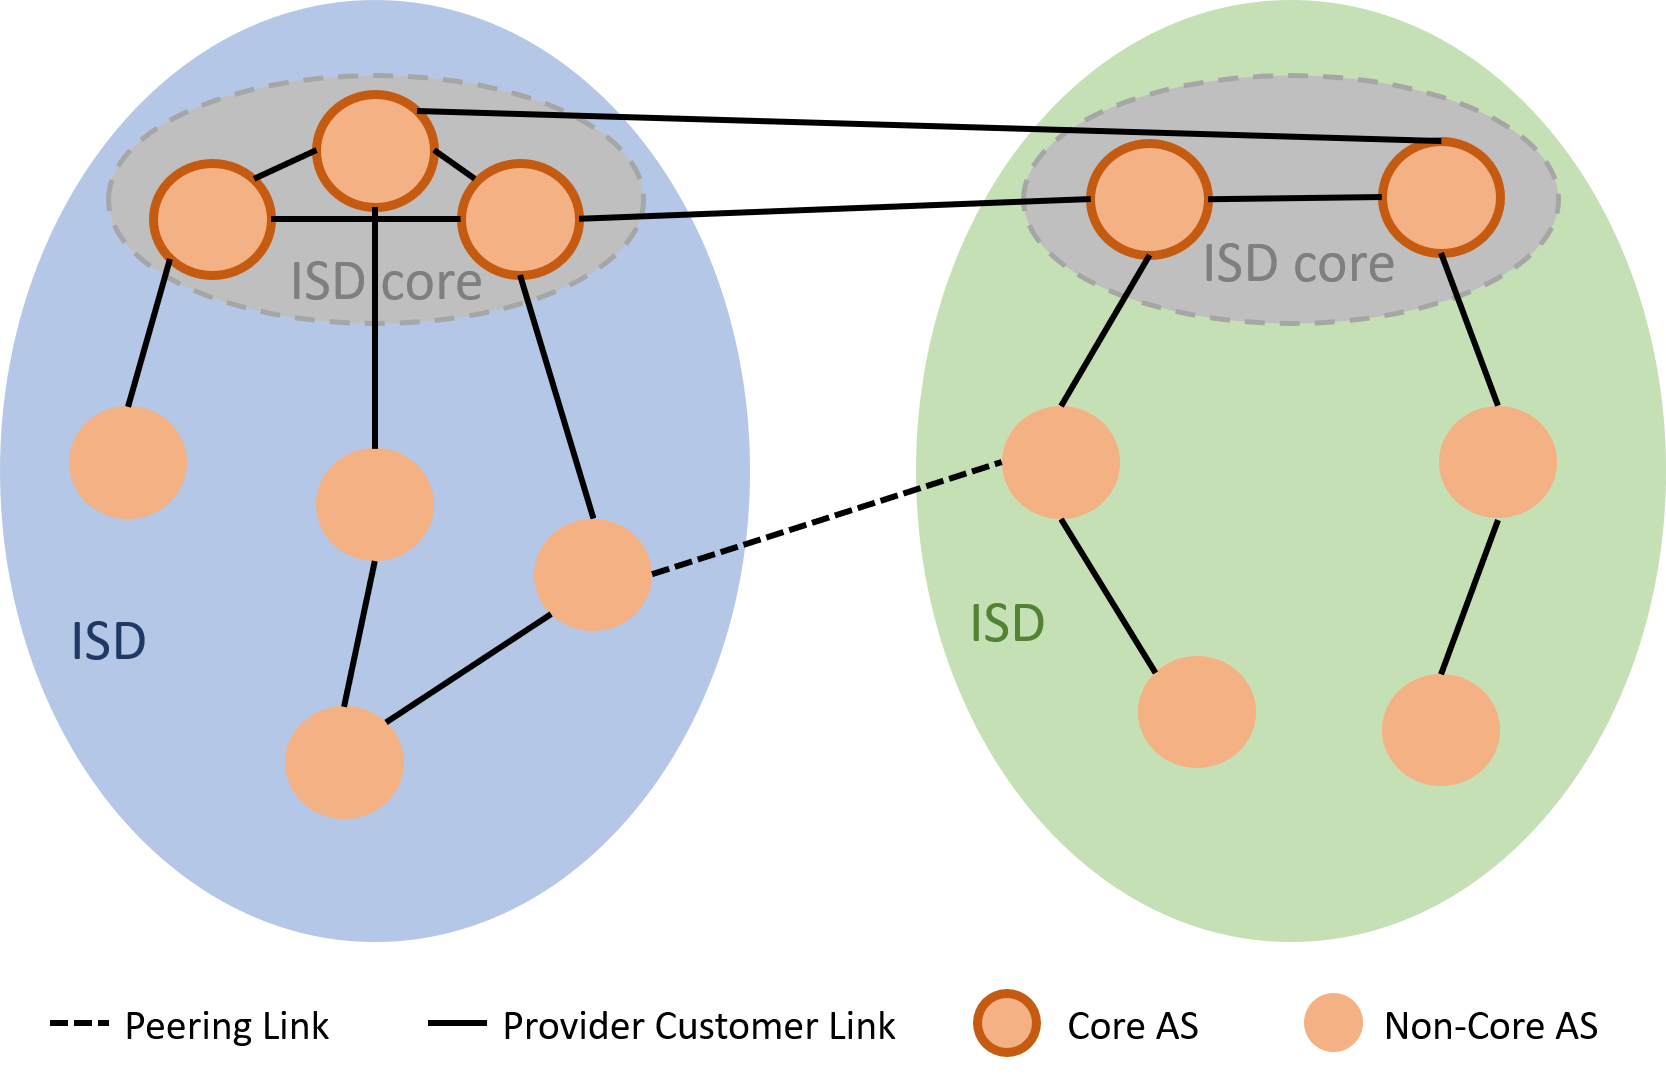
\includegraphics[width =\textwidth]{img/SCION-Topology.png}
	\caption{Basic SCION Topology}
	\label{Basic SCION Topology}
\end{figure}

\section{SCIONLab}
\acs{SCIONLab} is the distributed testbed for \acs{SCION}. Most of the network is managed by the Network Security Group of \acs{ETH} Zurich. The \acsp{AS} that are not managed by \acs{ETH} Zurich are called user-\acsp{AS}. Each of them is typically attached to one of the few \aclp{AP} that are part of the network infrastructure managed by \acs{ETH}. The \acsp{AP} are the only \acsp{AS} that allow direct connections to user-\acsp{AS}.
\\
The \acs{SCIONLab} network consists of multiple \acsp{ISD}, most of which are grouping together \acsp{AS} based on their geographic location or membership of a political union. However, one \acs{ISD} has the purpose of building a backbone for the entire \acs{SCIONLab} network. It is heavily interconnected and is hosted on \aclp{AWS}.

\subsection{SCIONLab as an Overlay Network}

Each \acs{SCIONLab}-\acs{AS} is based on a  \acs{VM} (currently running Ubuntu-16.04), a container or a dedicated \acs{SCION} system. Each \acs{SCIONLab}-\acs{AS} has to at least have the following services available: 
\\
\begin{enumerate}
\item A \textbf{\acl{BS} (\acs{BS})} that sends and receives the \acsp{PCB}
\item A \textbf{\acl{PS} (\acs{PS})} that stores the path segments and disseminates them to the customers.
\item A \textbf{\acl{CS} (\acs{CS})} that holds the certificates which are used to validate the paths.
\item A \textbf{\acl{BR} (\acs{BR})} that routes (on a \acs{SCION}-level) the traffic leaving the \acs{AS}.
\end{enumerate}

As shown in figure \ref{SCIONLab-AS} the \acl{BR} is also responsible for wrapping the \acs{SCION}-traffic into \acs{IP}-traffic. This is simply done by setting up an \acs{IP}-connection to the corresponding \acl{AP} and then send the \acs{SCION} packets over that connection. It is important to note that the \acl{BR} doesn't do any routing on an \acs{IP}-level.

\begin{figure}[h]
	\centering
	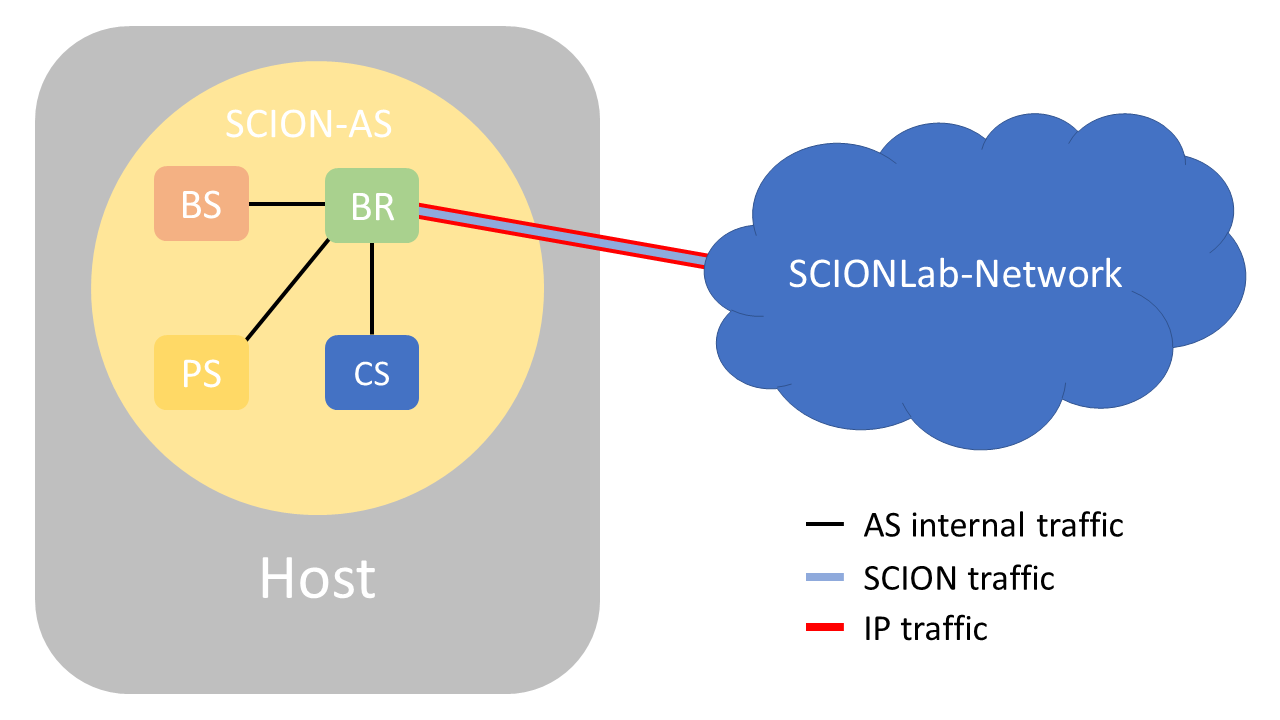
\includegraphics[width=\textwidth]{img/SCIONLab-AS.png}
	\caption{Schematic representation of a minimal SCIONLab-AS set-up}
	\label{SCIONLab-AS}
\end{figure}

\newpage

\subsection{SCIONLab AS}
There are two main ways to set up a \acs{SCIONLab}-\acs{AS}. The most common one is to set it up in a \acs{VM}. The other option is to set it up on a dedicated \acs{SCION} system. Either way, you can do that by creating an account on \href{https://www.scionlab.org}{scionlab.org} and use the web interface to configure your \acs{AS} to your needs. This web portal is called \acs{SCIONLab} Coordination Service. After you configured your \acs{AS}, you can download the files that are used to either set up the \acs{VM} or the dedicated \acs{SCION} system. The \acl{AP} needs some time to receive the new configuration files to set up the connection to the user-\acs{AS}. When the \acs{AP} is ready, you will receive an e-mail that informs you about it. As visible in figure \ref{SCIONLab Coordination Service} the current version of the \acs{SCIONLab} Coordination Service doesn't allow you to configure any bandwidth limits.

\begin{figure}[h]
	\centering
	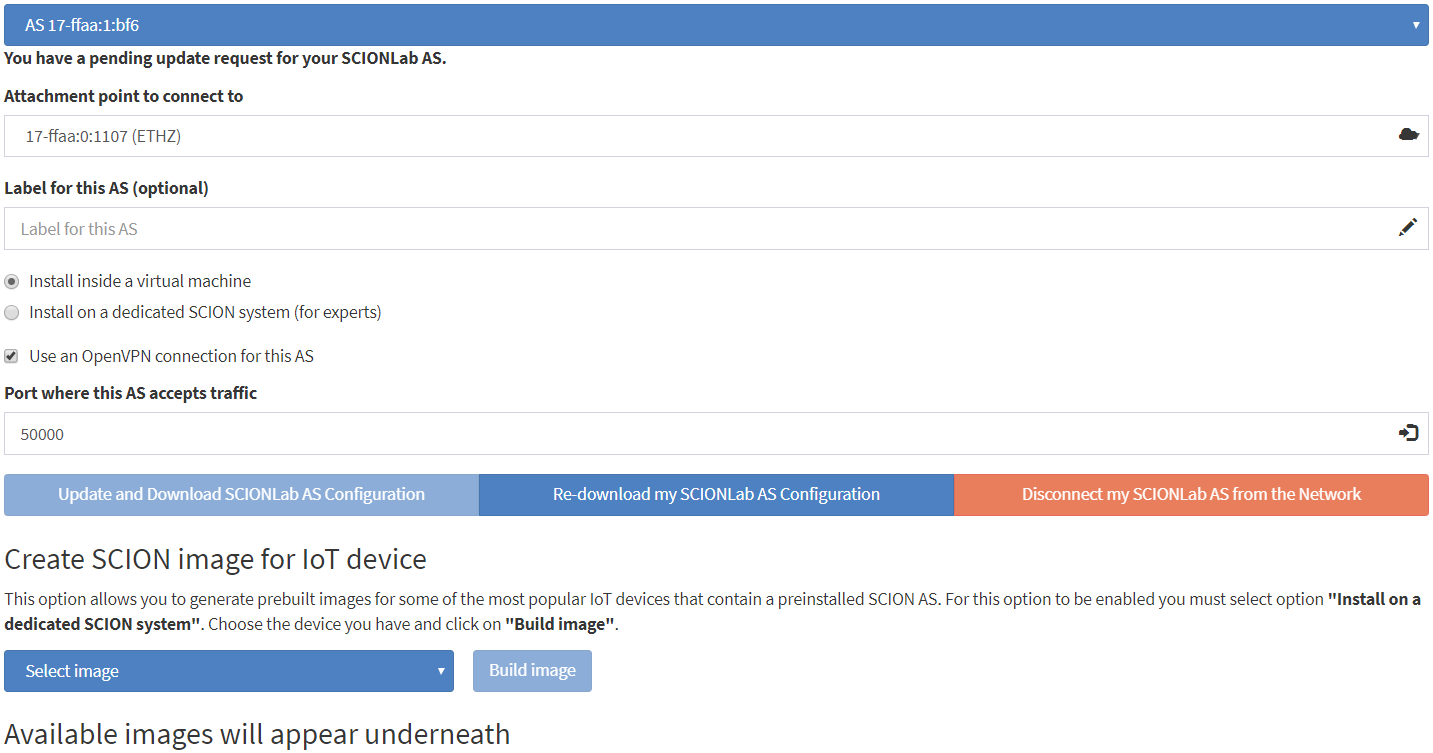
\includegraphics[width=\textwidth]{img/SCIONLab_Coordination_Service.png}
	\caption{Web Interface of the SCIONLab Coordination Service }
	\label{SCIONLab Coordination Service}
\end{figure}

\newpage

\subsection{Topology}
%TODO check if right
Figure \ref{Basic SCIONLab Topology} shows how the \acs{SCIONLab}-Network is set up. The user-\acsp{AS} are hosted by the users and connect to \acs{SCIONLab} by setting up a connection to an \acs{AP}. By doing so, the user-\acs{AS} automatically joins the \acl{AP}s \acs{ISD}. Infrastructure-\acsp{AS} are \acsp{AS} that are permanently connected to the \acs{SCIONLab}-Network and take part in routing and forwarding packets according to the \acs{SCION} protocol (\acsp{AP} are infrastructure-\acsp{AS} as well). Even though it's not shown in figure \ref{Basic SCIONLab Topology} the \acsp{AS} of \acs{SCIONLab} are of course also grouped into \acsp{ISD}. The only difference between \aclp{AP} and other infrastructure-\acsp{AS} is that \acsp{AP} allow connections to user-\acsp{AS}, while the normal infrastructure-\acsp{AS} don't.

\begin{figure}[h]
	\centering
	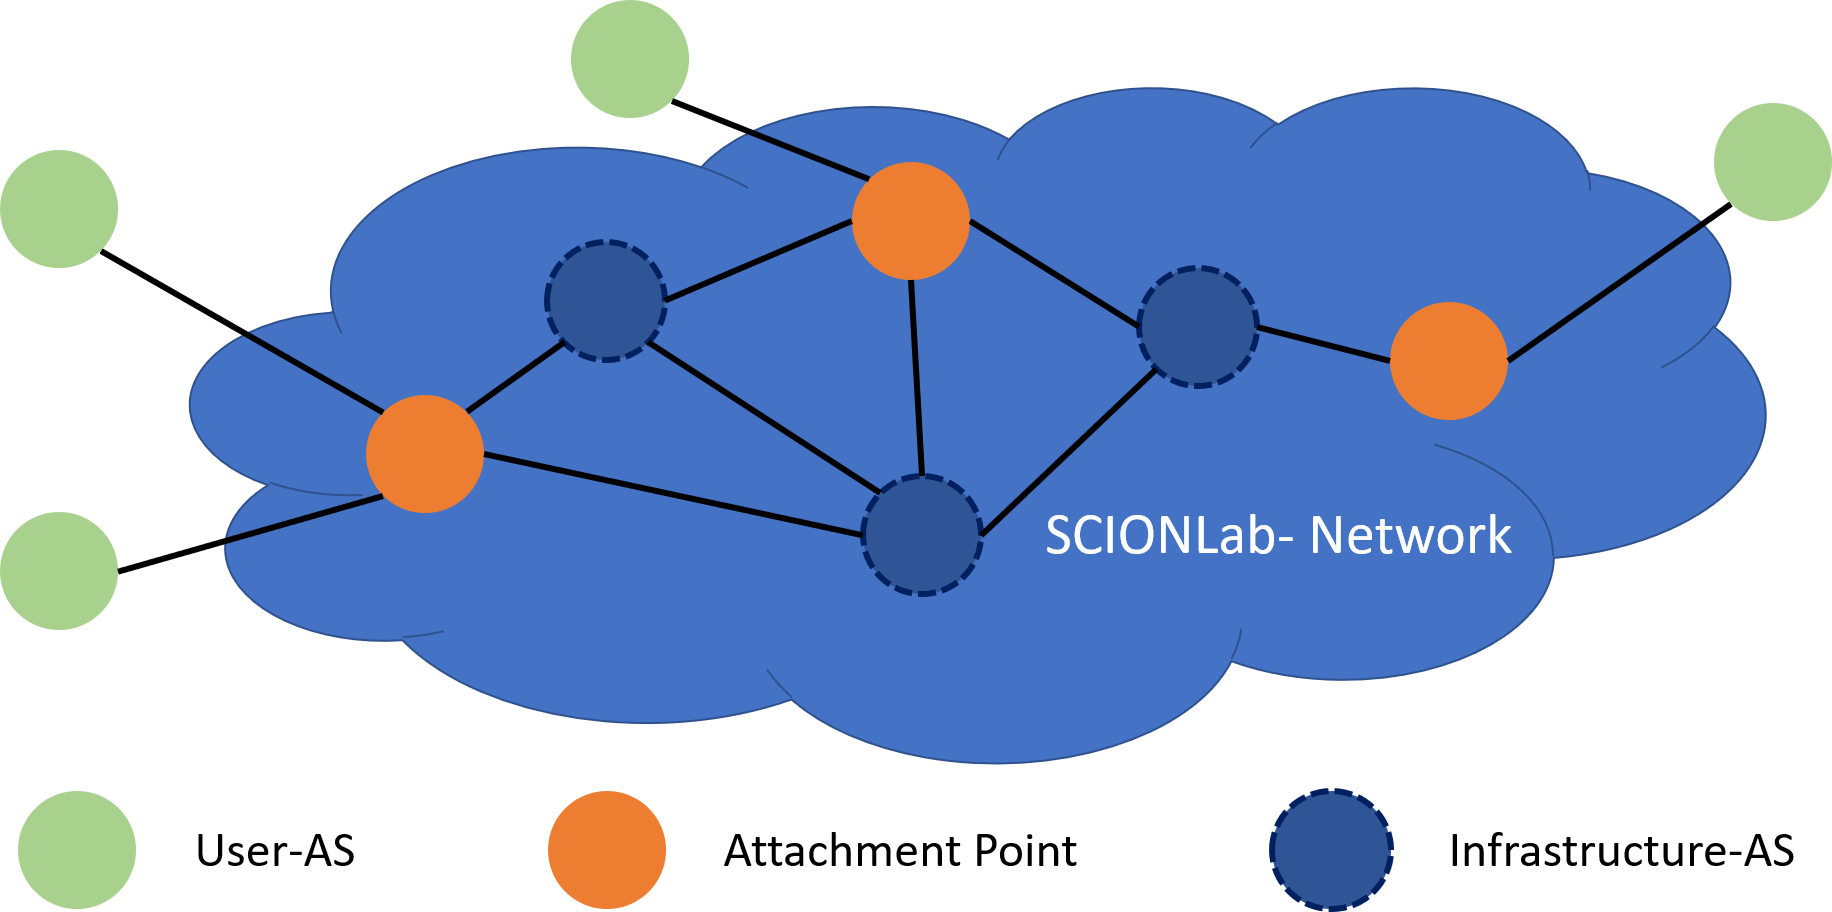
\includegraphics[width =\textwidth]{img/SCIONLab-Topology.png}
	\caption{Basic SCIONLab Topology}
	\label{Basic SCIONLab Topology}
\end{figure}

\chapter{Traffic Control}
Traffic control in Linux is realized using a tool named \acs{TC}. It consists of four basic techniques.

\begin{enumerate}
\item \textbf{Shaping}: This is the technique we will be using in order to enforce an upper bandwidth limit. But in general, it is the process of manipulating the bandwidth. It can also be used to smooth out bursts in order to improve the quality of service. Shaping is done on egress traffic.

\item \textbf{Scheduling}: This is the process of staging packets according to a schedule. Like this reordering of packets can be achieved. Scheduling as well happens with egress traffic.

\item \textbf{Policing}: This is the equivalent to shaping but for ingress traffic. It is worth noticing that traffic policing is more limited than traffic shaping, since there is no ingress queue.

\item \textbf{Dropping}: This is a quite primitive approach of just dropping traffic that exceeds a given bandwidth. This is applicable for both ingress and egress traffic.
\end{enumerate}

For our needs, traffic shaping fits best. But since we need to limit ingress traffic as well, and shaping only operates on egress traffic, we need a workaround. More about that in section  \ref{Ingress Traffic}. Traffic control using \acs{TC} is implemented using three basic building blocks: \acp{QDISC}, classes and filters. They will be discussed in section \ref{TC}.

\section{Theory}
\subsection{Traffic Shaping}
As previously stated, traffic shaping happens with egress traffic. However, there is a special \acs{QDISC} that is handling ingress traffic. Since this \acs{QDISC} is the only one applicable on ingress traffic, it is called \textit{ingress}. The term \acl{QDISC}, in that case, is a bit misleading, because there is no such thing as an ingress queue. All the other \acsp{QDISC} handle egress traffic and are quite diverse. Each \acs{QDISC} has a shaping algorithm that shapes the traffic passing the corresponding \acs{QDISC}. \acsp{QDISC} can be either classful or classless (the ingress \acs{QDISC} is the latter). Classful \acsp{QDISC} have a shaping algorithm that can handle traffic, which is classified in different classes, differently. Both the classes and the classifiers, which are filters that determine which kind of traffic belongs to which class, are attached to the \acs{QDISC}. Classless \acsp{QDISC} can obviously not handle classes. However they can handle filters, which can either do policing on the traffic or i.e. redirect it to a different interface.

\subsection{Egress Traffic}
To enforce a bandwidth limit per \acs{IP} connection it makes sense to use a classful \acs{QDISC}, because this provides us with the flexibility to configure the classes exactly according to our needs. The best choice for a classful egress \acs{QDISC} that allows us to enforce bandwidth limits, seems to be an \ac{HTB}-\acs{QDISC}, which is based on the \ac{TBF} shaping algorithm. The \acs{TBF} algorithm roughly works as follows: 
\\There is a bucket that holds tokens. Every token corresponds to approximately one byte. Whenever a packet arrives, the \acs{TBF} algorithm tries to consume as many tokens out of the token bucket as there are bytes in the packet. If there are enough tokens, then the packet can be sent at full speed. If there are not enough tokens, then the packet gets enqueued and has to wait until there are again enough tokens in the bucket. The bucket is constantly being filled with tokens at the rate we configured. Like this the bandwidth can be limited in average and at the same time allow short bursts at maximum speed, where the size of these bursts depends on the size of the bucket. It is worth noticing, that the limitation looses in accuracy if the limit is above 1mbit/s. But the accuracy loss shouldn't be too severe for our use-case.
More about the \acs{HTB}-\acs{QDISC} can be found in section 9.5.5. of \textit{Linux advanced routing \& traffic control HOWTO}\cite{hubert2002linux}.

\newpage
\subsection{Ingress Traffic} \label{Ingress Traffic}
There is only one \acs{QDISC} that can handle ingress traffic, namely the ingress \acs{QDISC}, which is classless. Since it is classless we can't do traffic shaping per \acs{IP} connection as easily as we do it with egress traffic. Therefore we are left with two options:
\begin{enumerate}
\item \textbf{Traffic policing using filters}:
\\With this option we can only use the configuration options \acs{TC}-filters provide. The filters would be directly attached to the ingress \acs{QDISC}. Since these policing options are a bit limited and not as powerful as the shaping options, we are not going to use policing.
\item \textbf{Traffic shaping using virtual interfaces}:
\\The option of using virtual interfaces gives us the same configuration possibilities as we have with egress traffic. At the ingress \acs{QDISC} we simply attach one filter that redirects all the traffic it receives to a virtual interface, on which we then have a \acs{HTB}-\acs{QDISC} and therefore have the same options as we have with the \acs{HTB}-\acs{QDISC} that handles egress traffic. You can think about this the following way: The virtual interface sends the ingress traffic to the host and therefore the ingress traffic becomes egress traffic from the perspective of the virtual interface. Figure \ref{Interface set-up} should make that clearer. Since this option is more powerful, in the sense that we have more shaping options, this is our option of choice.
\end{enumerate}

\begin{figure}[h]
	\centering
	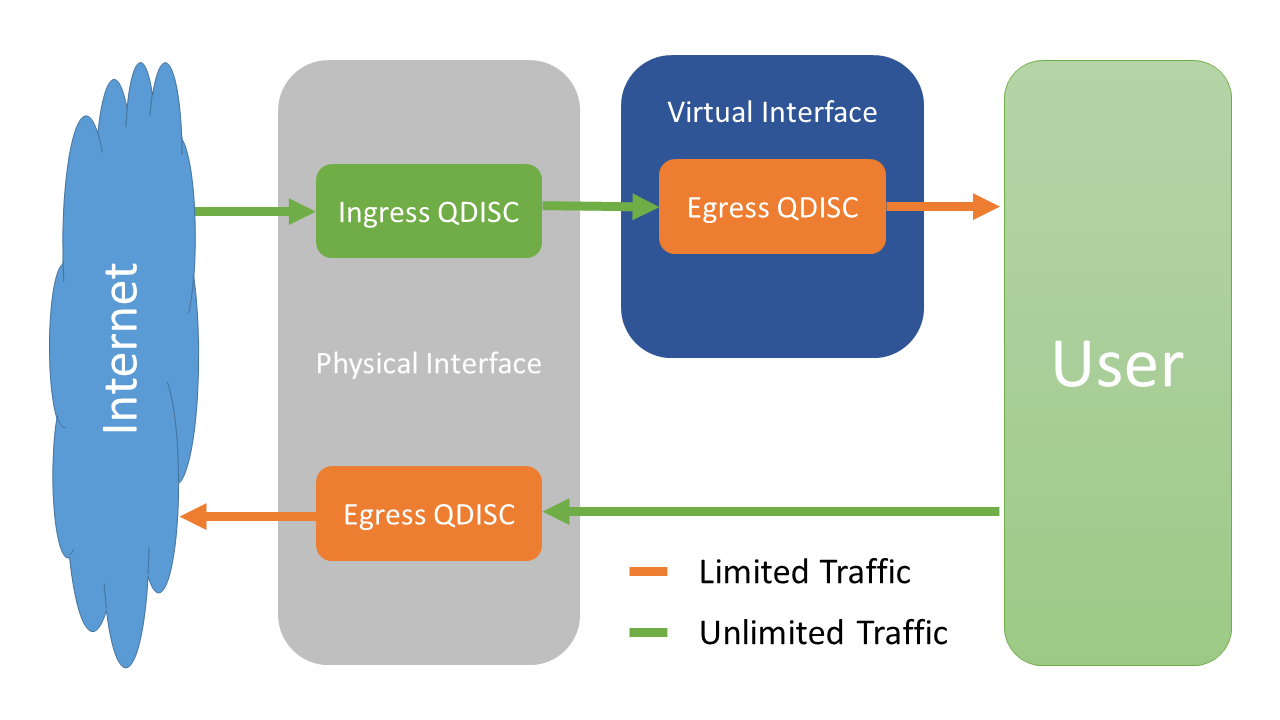
\includegraphics[width=\textwidth]{img/Interface-Setup.png}
	\caption{Interface set-up}
	\label{Interface set-up}
\end{figure}

\section{TC} \label{TC}
\acs{TC} is a state of the art traffic control tool that is part of the iproute2 utility package and is by default installed on all \aclp{AP}. It can handle traffic based on any properties that can be found in the \acs{IP}-header, as well as marks that were set using iptables or ipchains.

\subsection{Queuing Disciplines}

A \acs{QDISC} or \acl{QDISC} is the controlling unit that sits between the kernel and the interface. Whenever the kernel wants to send something to an interface, it enqueues it via the \acs{QDISC} attached to the interface. The kernel then immediately tries to get as many packets as possible from the \acs{QDISC} in order to send them to the network adapter driver. The \acs{QDISC} can therefore decide in what manner it allows the kernel to get the packets back in order to send them. This also makes it clearer why there are very sophisticated egress \acsp{QDISC}, while there is only one very primitive ingress \acs{QDISC}.
\\
As previously mentioned, \acsp{QDISC} can be either classful or classless. If we want to do more than just simple policing or dropping then it is recommended to use classful \acsp{QDISC}, simply because classful \acsp{QDISC} can be configured more precisely, which makes them more powerful.

\subsection{Classes}

Classes are used to configure classful \acsp{QDISC}. They are mostly used to handle a subset of the entire traffic. Which kind of traffic belongs to that subset is determined by classifier filters, which are attached to the parent \acs{QDISC}. Each class has exactly one leaf \acs{QDISC}, to which there can again be classes attached. Like this classes and \acsp{QDISC} can build up a hierarchy tree, which is then propagated from top to bottom, namely from the root \acs{QDISC} to the leaf \acs{QDISC}.

\subsection{Filters}
There are two main types of filters:
\begin{enumerate}
\item \textbf{Classifiers:} They map traffic based on some metric to a class of a classful \acs{QDISC}, where the traffic is then further handled according to the leaf \acs{QDISC}
\item \textbf{Policers:} They are used to directly manipulate traffic. In our case we use them to redirect traffic from the ingress \acs{QDISC} to a virtual interface. But they can also be used to directly limit the bandwidth, however without the configuration options a classful \acs{QDISC} provides.
\end{enumerate}
\chapter{Conception}
In order to conceptualize the bandwidth limiter for \acs{SCIONLab} properly, we first need to formalize the requirements. We want to achieve the following:

\begin{enumerate}
\item[$\bullet$]The \acs{SCIONLab} administrators should be able to set a maximal bandwidth that is available to the user-\acsp{AS}.
\item[$\bullet$]The users should be able to set an upper limit for the bandwidth in the range of $[0,x]$ where $x$ is the bandwidth limit set by the \acs{SCIONLab} administrators.
\item[$\bullet$] The above mentioned limits should be enforced automatically by only making configurations on the \acsp{AP}.
\end{enumerate}

We split up these three requirements into two sections. The first two belong to the front end of the project, where as the third requirement is part of the back end.

\section{Front End}

The front end part of the project is all about the \acs{SCIONLab} server. The implementation of that server can be found on \href{https://github.com/ManuelMeinen/scionlab/tree/bw-limit}{github.com}\cite{meinen2019scionlab}. There is already a configuration page, where the users can set the desired configuration for their user-\acsp{AS}. On the same configuration page we simply add a field, where the users can insert a bandwidth limit between 0 and the limit set by the \acs{SCIONLab} administrators. Other bandwidth limits get already rejected by the form.
\\
The \acs{SCIONLab} server stores information about the entire topology of the \acs{SCIONLab} network, including information about the links from the \acsp{AP} to the user-\acsp{AS}. Per link there is a field that stores the maximal bandwidth for that link. This field already exists but is currently not used. Therefore we simply set that attribute to the bandwidth limit that the user chose.
\\
The \acs{SCIONLab} server regularly generates files according to its data model that are then sent to the \acsp{AP}, in order to configure them for newly added or updated user-\acsp{AS}. These files are packed in a tarball and then delivered and unpacked on the \acsp{AP}. We can use this mechanism to deliver the information we need to the \acsp{AP}, in order to enforce the bandwidth limitations. So we simply add a \ac{JSON}-file called \textit{link\_info.json} to that tarball, which holds the information we need to perform bandwidth limitations.

\section{Back End}

The back end part is all about configuring the \acsp{AP} in a way that the bandwidth limits that are specified in the \textit{link\_info.json} file are put into effect. We do that using the \acs{TC} utility. However, there is no \acs{API} to use \acs{TC} in an automated way. Therefore we need to write a wrapper program that configures \acs{TC} via the command line. This wrapper program is written in Python and is available on \href{https://github.com/ManuelMeinen/SCIONLab_Bandwidth_Limiter}{github.com}\cite{meinen2019scionlabBwLimiter}. Further details on how this program is implemented can be found in chapter \ref{Implementation}.
\\
Furthermore, we have to make some design decisions. Especially, we have to decide on how to build up the \acs{TC} logic. Figure \ref{QDISC-Set-up} shows in an abstract way how \acsp{QDISC}, classes and filters are set up on both physical as well as virtual interfaces and how they are related.
\\
Ingress, as well as egress traffic, firstly goes through the physical interface. Ingress traffic is then redirected by the \textit{ingress} \acs{QDISC} (with handle ffff) to a virtual interface. On the virtual interface, ingress traffic is handled the same way as egress traffic is on the physical interface. In both cases we use an \acs{HTB}-\acs{QDISC}. To make these \acsp{QDISC} more distinguishable, we define the handle for a \acs{QDISC} on a physical interface to be 1 and 2 if it is on a virtual interface. In both cases we define one class for each connection to a user-\acs{AS} and set the corresponding bandwidth limit to its leaf-\acs{QDISC}. Furthermore we define a default class, which limits all traffic going through this interface that doesn't match with any filter to the default bandwidth. Each class has the \acs{AS}-id as a class id, which is unique to each \acs{AS}. The default classes have a class id of 9999. Each \acs{HTB}-\acs{QDISC} has as many classifier filters as there are user-\acsp{AS} plus one implicit one for the default class (represented as arrows in figure \ref{QDISC-Set-up}). The \textit{ingress} \acs{QDISC} has only one filter, which is a redirect filter that redirects ingress traffic of the physical interface to the virtual interface.
\begin{figure}[h]
	\centering
	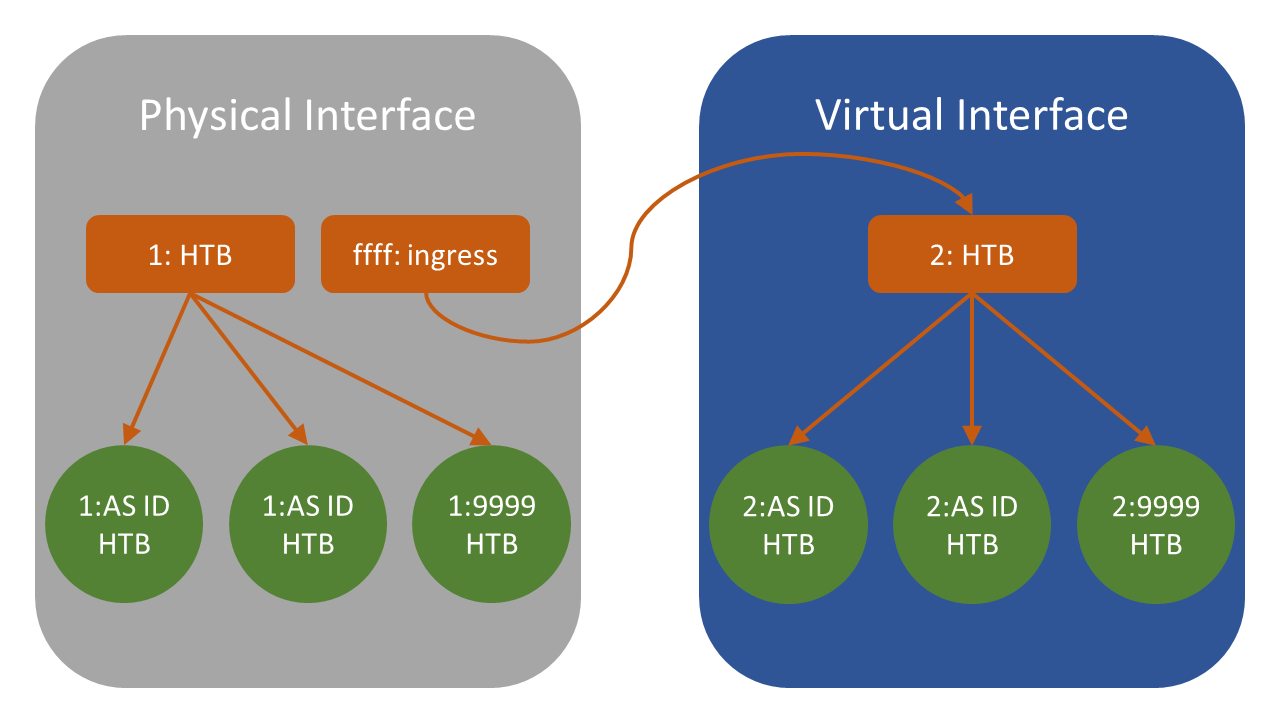
\includegraphics[width=\textwidth]{img/QDISC-Set-up.png}
	\caption{QDISC/Class hierarchy}
	\label{QDISC-Set-up}
\end{figure}
\chapter{Implementation} \label{Implementation}

\section{Front end}



\section{Back end}

The back end consists mainly of the python files listed below. Additionally there are some \acs{JSON}-files that are used to either safe some settings or store some text that would take up too much space in the code and is therefore put into a separate file for the sake of readability. The python files have the following functionality:

\begin{enumerate}
\item[$\bullet$]\textit{scionlab\_bw\_limiter}:
\\
This file implements the entry point of the entire program. It parses command line arguments, let's you configure the default bandwidth and the path to the \textit{link\_info.json} file and invokes the \textit{bandwidth\_configurator.py} in order to enforce or reset bandwidth limitations or to show the current \acs{TC} configuration. It accepts the following options:
	\begin{enumerate}
	\item[\textit{-h}:] Show help text that explains how to use the program. This text is stored in the \textit{config\_files/help.json} file.
	\item[\textit{-l}:] Enforce the bandwidth limitations according to the \textit{link\_info.json} file.
	\item[\textit{-r}:] Reset any previously set \acs{TC} configurations.
	\item[\textit{-s}:] Show the current \acs{TC} configuration.
	\item[\textit{-b}:] Set or update the default bandwidth. This takes as an argument a positive integer, which represents the default bandwidth in kilo bits per second.
	\item[\textit{-p}:] Set or update the path to the \textit{link\_info.json} file. This option takes the path to that file as an argument.
	\end{enumerate}

\item[$\bullet$]\textit{code\_base/bandwidth\_configurator.py}:
\\
This file contains the implementation of the \textit{limit()}, \textit{reset()} and \textit{show()} functions. The \textit{limit()} function reads in the \textit{link\_info.json} file and creates link objects accordingly. Then it sets up the virtual interfaces, creates the \acs{TC} logic and invokes the \textit{make()} function from the \textit{tc\_logic.py} file. The \textit{reset()} function simply deletes the root \acs{QDISC} as well as the ingress \acs{QDISC} for each used interface. And finally the \textit{show()} function is responsible for printing out the current \acs{TC} configuration.

\item[$\bullet$]\textit{code\_base/cmd\_executor.py}:
\\
The command executor implements some static helper functions, that simplify running a command on the command line. One function silently runs a command using the subprocess \acs{API}, an other one runs a command and prints it to the console, one runs the command silently but returns the output it received by running the command and finally one function runs a command after it printed it and returns the output.

\item[$\bullet$]\textit{code\_base/constants.py}:
\\
This file contains some static variables that are constant throughout the entire program. 

\item[$\bullet$]\textit{code\_base/interfaces.py}:
\\
This file is used to retrieve information about the interfaces configured on the host machine and bundle it together in interface objects.

\item[$\bullet$]\textit{code\_base/links.py}:
\\
Analogously to the \textit{interfaces.py} file the \textit{links.py} file is used to bundle together information about links. This information is parsed form the \textit{link\_info.json} file. Furthermore, in this file the virtual interfaces are set up and mapped to their corresponding physical counterpart.

\item[$\bullet$]\textit{code\_base/systeminfo.py}:
\\
The \textit{systeminfo.py} file is used to retrieve some information about the host like whether a file exists or which interface is used by default.

\item[$\bullet$]\textit{code\_base/tc\_command\_generator.py}:
\\
The \acs{TC} command generator is used to generate the \acs{TC} commands that are used in order to configure the system. The generation functions return these commands as strings. They are later executed using the command executor.

\item[$\bullet$]\textit{code\_base/tc\_logic.py}:
\\
This file is the centrepiece of the entire program. It defines the building blocks to build up the entire logic of our \acs{TC} hierarchy according to figure \ref{QDISC-Set-up}. The \ac{UML}-model in figure \ref{tc logic uml} visualizes the relevant building blocks and their attributes and functions. The most interesting function is probably the \textit{make()} function. It first uses the \acs{TC} command generator to get the command to turn it's properties into \acs{TC} configurations, executes the command using the command executor and then recursively calls \textit{make()} on the building blocks that are lower down in the hierarchy tree. Like this the entire \acs{TC} logic can be turned into \acs{TC} configuration on the host. 

\item[$\bullet$]\textit{code\_base/virtual\_interfaces\_manager.py}:
\\
The virtual interface manager is used to set up and delete the virtual interface and to map them to their physical counterparts.

\end{enumerate}

\begin{figure}[h]
	\centering
  	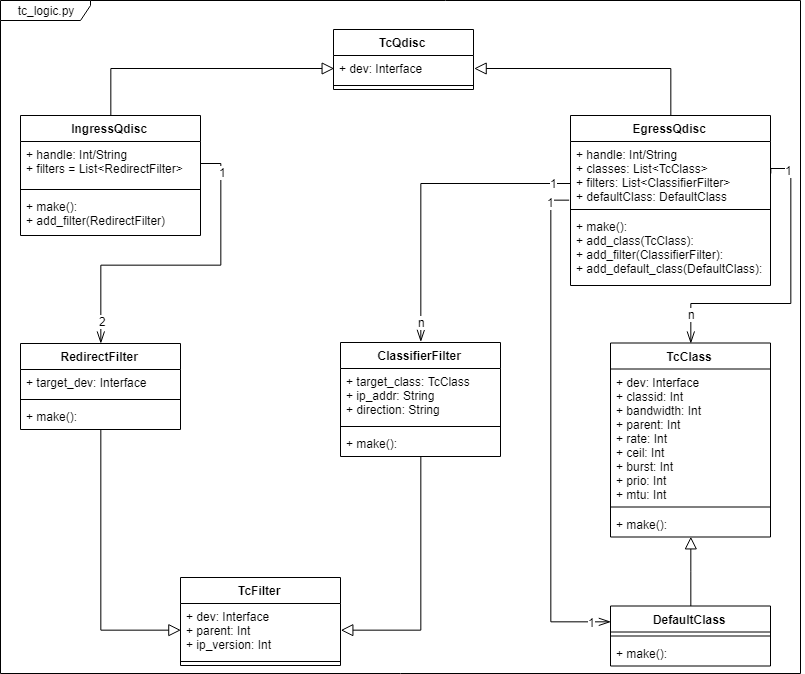
\includegraphics[width=\textwidth]{img/tc_logic_uml.png}
    \caption{UML-Model of \text{tc\_logic.py}}
    \label{tc logic uml}
\end{figure}

\chapter{Evaluation}
Evaluating the results of bandwidth limitations is more difficult than it might seem. Both, bandwidth limitation utilities like \acs{TC} as well as testing tools like iPerf3 are often hard to configure correctly and are sometimes documented quite incomprehensibly. Therefore, it is often unclear whether errors are measurement errors or limitation errors. Furthermore, there is no such thing as standard \acs{IP}- or even \ac{UDP}-traffic. Packets can have different sizes, can be reordered or get lost. All those factors can influence and sometimes falsify the measurement. And finally it is questionable whether the traffic that is generated by the testing tools is similar enough to normal traffic generated by an \acs{AS}, such that we can conclude anything meaningful.
\\
What is known about the environment in which the \textit{scionlab\_bw\_limiter} will be running is that we deal with \acs{UDP}-traffic over \acs{IP}v4 and at some point in the future might be dealing with \acs{IP}v6 traffic as well. Therefore, we mainly focus on testing the bandwidth limitations using \acs{UDP}-traffic over \acs{IP}v4. However, note that the \textit{scionlab\_bw\_limiter} also works with \acs{IP}v6 traffic and that the test results look almost identical to the test results when using \acs{IP}v4 traffic.

\section{Test Set-up}

As a test set-up it makes sense to have a test server, which doesn't have any bandwidth limitations and a test client, where the \textit{scionlab\_bw\_limiter} will enforce the desired bandwidth limits. As a test client I decided to use my development \acs{VM}, which I also use to develop and test the \textit{scionlab\_bw\_limiter}. This \acs{VM} runs Ubuntu 18.04, which is a newer version than the one running on the \aclp{AP}, but since \acs{TC} works the same way on both versions of Ubuntu, this should not matter. The test server is a Ubuntu 18.04 server that runs in a \acs{VM} as well and is hosted on the same physical machine as the test client. Therefore traffic between the test server and the test client is not real network traffic, but since the \acs{TC} configurations are effective between the Linux kernel and the network driver, where both of which are virtualized, the \acs{TC} configurations should have the exact same effect in this setting as in the real environment.
\\
For testing the bandwidth between the test client and the test server, I chose two different approaches, one of which turned out to be quite useless, whereas the other one seemed to be reasonable.

\subsection{Naive Approach}
%TODO get rid of that one
In the beginning it was not that easy to figure out how iPerf3 had to be configured and how the test results were to be interpreted. Therefore I decided to take a simpler approach in order to get an idea on what I should expect from the iPerf3 test results. 
\\
I decided to simply generate a file of a certain size, send it either from the server to the client or the other way around and measure the time it takes until it arrives at the other end. Unfortunately it's not that simple. The connection between the two \acsp{VM} is quite fast, even when its bandwidth is limited. However relative to the transmission time, the time to load a file from memory or even from the harddisk is quite long. Therefore the measurements were highly inaccurate.

\subsection{Using iPerf3}

Since the naive approach turned out to be to inaccurate to be of any use, I decided to set up an iPerf3 test environment. I installed iPerf3 on both the test client as well as on the test server and let the test server run iPerf3 as a server. Note that the same software is used for both the server side as well as the client side. They just run in different modes. On the client I can now connect to the test server and run highly customisable tests with the server. Normally the client is the one sending data to the server, but iPerf3 can be run in a reverse mode (using the \textit{-R} option), such that we can test both ingress as well as egress traffic without having to switch between client and server mode on our machines.

\section{iPerf3}

iPerf3 is a state of the art network performance measurement tool. It is a successor of iPerf and iPerf2. However it has been completely rewritten in order to make the code base cleaner and simpler and is therefore not backward compatible with iPerf2. iPerf3 has been developed by \ac{ESnet}, which is a high-speed computer network provider for the United States Department of Energy. iPerf3 is open-source and can be found on \href{https://github.com/esnet/iperf}{github.com}\cite{mah2018iperf3}.
\\
iPerf3 can test both \ac{TCP} as well as \acs{UDP} traffic. In our case we only need to test \acs{UDP} traffic. This can be done by passing the option \textit{-u} as an argument to iPerf3. When running it we need to specify a target bandwidth (option \textit{-b}). iPerf3 then tries to achieve this bandwidth by sending traffic out at this rate. To run iPerf3 in server mode we only have to pass \textit{-s} as an argument. For running it in the client mode we have to analogously pass the \textit{-c} option followed by the server's \acs{IP}-address. Last but not least, we can optionally set the buffer length of the buffer from which is sent and to which is received by passing the option \textit{-l} followed by a size in bytes as an argument. As we will see in section \ref{Test Results}, this option is of quite a significance.

\section{Test Results}\label{Test Results}
%TODO figure out what l realy means and why it influences the bandwidth
The following test results occurred under the following configuration:
\\
The server's \acs{IP}-address is in our case 192.168.17.129, the \acs{IP}-connection to the server is limited to 500Kbps and the default bandwidth is 1000Kbps. The \ac{MTU} parameter in \acs{TC} is set to the \acs{MTU} of the network interface that is used to connect to the specific \acs{IP}-address. In our case this is 1500 bytes. The burst parameter, which is the size of the bucket in the \acs{TBF} algorithm is set to 5K. The ceil rate is the same as the normal rate, which is 500Kbps to the test server and 1000Kbps to any other \acs{IP}-device that uses the same interface.
\\
\\
On the test server, we start iPerf3 using no other options than the \textit{-s} option, that makes iPerf3 run in server mode (see listing \ref{Test Server Command}). On the client side, we configure a bit more. We set the \textit{-u} option, in order to generate \acs{UDP} traffic as test traffic. The target bandwidth is set to 2Mbps (option \textit{-b}) and the only parameter that we are going to change for different tests is the buffer length (option \textit{-l}). We start at a buffer length of 1000 bytes and go up to 10000 bytes. And finally we set the \textit{-R} option in case we want to run the test in reverse mode, meaning that we test with ingress traffic. Listings \ref{Example Egress Test Command} and \ref{Example Ingress Test Command} show what these commands look like. Note that if we set the buffer size too small, we encounter an error. This happens because the packets arrive in a different order than they were sent. Therefore iPerf3 can't measure the bandwidth any more. This phenomenon is discussed on \href{https://github.com/esnet/iperf/issues/457}{github.com}\cite{mah2016iperfIssue} in the issues section of the iPerf source code.

\begin{lstlisting}[language=sh, caption = Test Server Command, captionpos=b, numbers=left, frame=single, breaklines=true, breakatwhitespace=true, showstringspaces=false, label=Test Server Command]
iperf3 -s
\end{lstlisting}
\newpage
\begin{lstlisting}[language=sh, caption = Example Egress Test Command, captionpos=b, numbers=left, frame=single, breaklines=true, breakatwhitespace=true, showstringspaces=false, label=Example Egress Test Command]
iperf3 -c 192.168.17.129 -u -b 2Mbit -l 1000
\end{lstlisting}

\begin{lstlisting}[language=sh, caption = Example Ingress Test Command, captionpos=b, numbers=left, frame=single, breaklines=true, breakatwhitespace=true, showstringspaces=false, label=Example Ingress Test Command]
iperf3 -c 192.168.17.129 -u -b 2Mbit -l 1000 -R
\end{lstlisting}

\subsection{Interpretation of the Test Results}

Figure \ref{Evaluation of the Bandwidth} shows the average bandwidth over ten samples for both ingress as well as egress traffic with respect to the buffer size. For the egress traffic the results look quite good. The average egress bandwidth lies slightly above the bandwidth limit. This is because we allow short bursts at a higher speed. Therefore, the limitations on egress traffic can be considered as effective and stable.
\\
However, for ingress traffic it is a bit a different story. That the ingress bandwidth is lower than the egress bandwidth is expected, because there is a slight overhead by redirecting ingress traffic from a physical interface to a virtual interface. So having a situation like we have it with a buffer length of 1000 bytes would be desirable. However, we can't ignore that by increasing the buffer length, the ingress bandwidth drops quite drastically. For getting on the bottom of this issue, let us consider figure \ref{Evaluation of the Bandwidth Drops}. This figure shows the number of samples at a bandwidth of zero depending on the length of the buffer. It is visible that the bigger the buffer, the more the ingress traffic suffers from samples with a bandwidth of zero. This phenomenon happens with egress traffic as well, but there it is much less significant. The increasing number of zero bandwidth samples shows that the decreased average bandwidth is not caused by a wrong limitation, since the samples that make it through are received at a bandwidth that is around the desired limit, but that for some samples either iPerf3 fails to do a measurement at all or something prevents the machine from receiving data for some time. To figure out whether these anomalies are the result of side effects the \textit{scionlab\_bw\_limiter} causes or are measurement errors of iPerf3, we need compare these results with results we get if we enforce bandwidth limits using a different tool.

\begin{figure}[h]
	\centering
	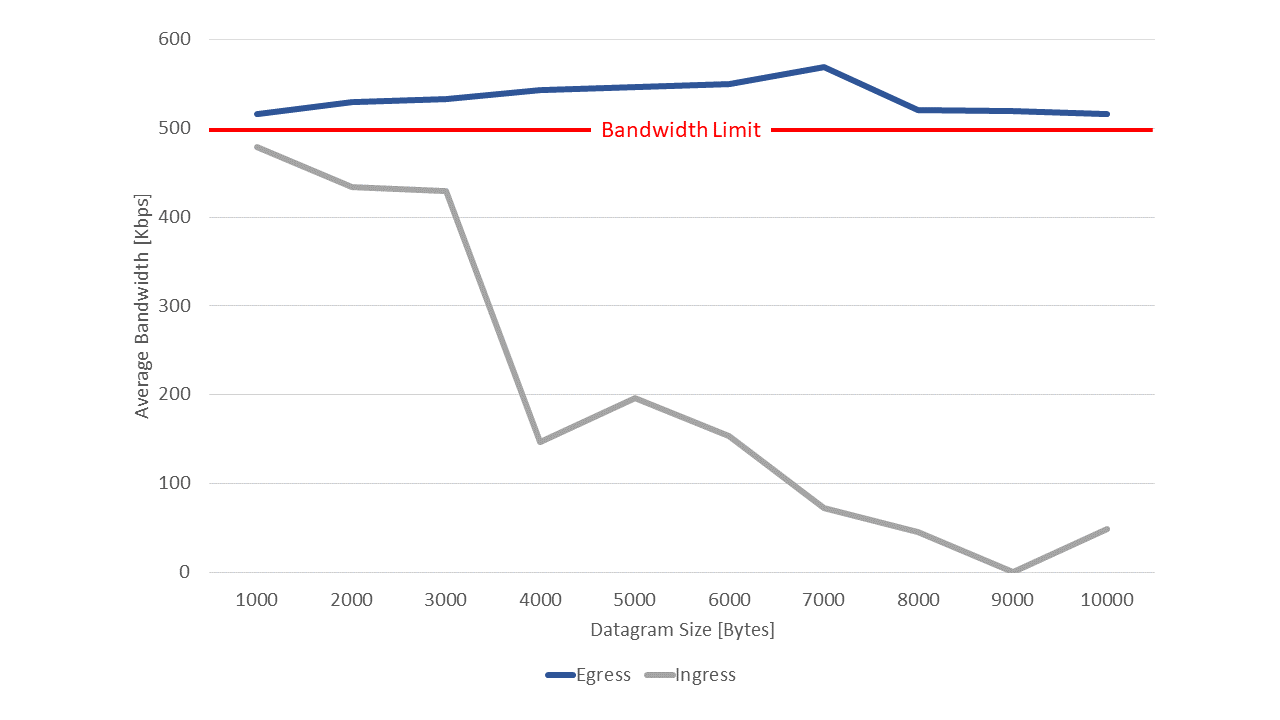
\includegraphics[width=\textwidth]{img/Evaluation-Bandwidth.png}
	\caption{Evaluation of the Bandwidth}
	\label{Evaluation of the Bandwidth}
\end{figure}

\begin{figure}[h]
	\centering
	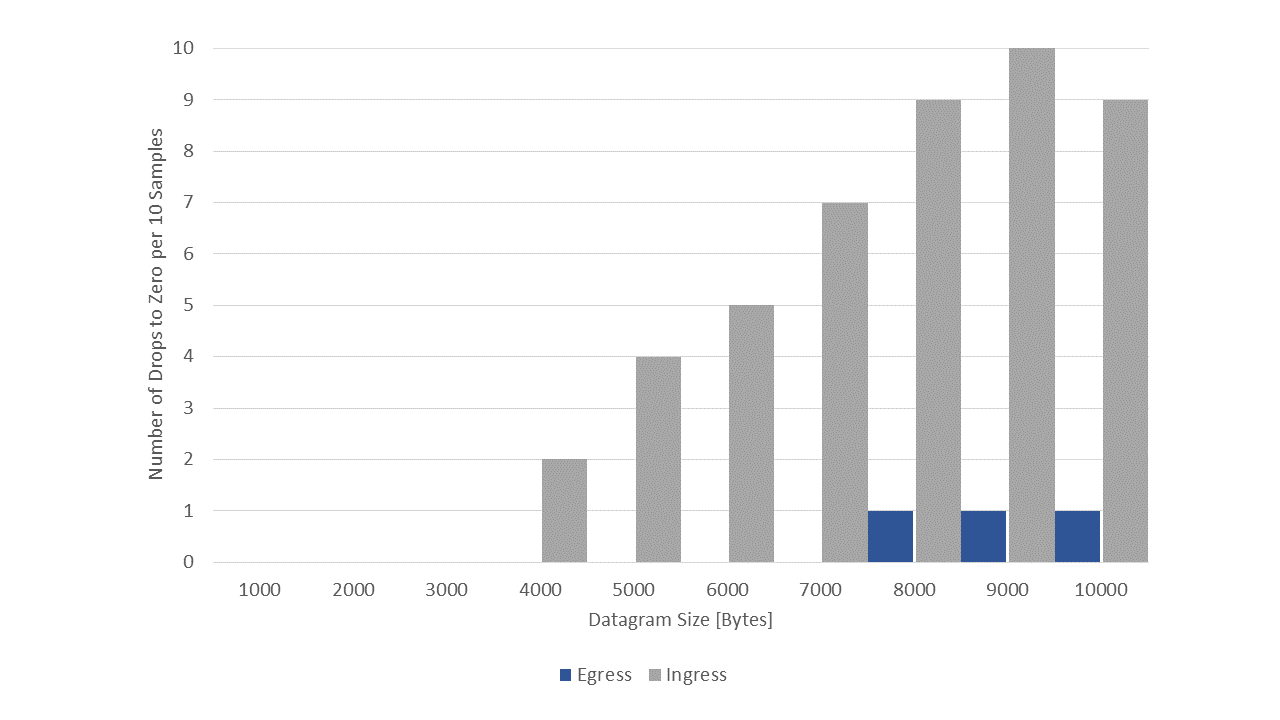
\includegraphics[width=\textwidth]{img/Evaluation-Zeros.png}
	\caption{Evaluation of Bandwidth Drops}
	\label{Evaluation of the Bandwidth Drops}
\end{figure}
%TODO maybe there is a better solution to layout that stuff...
\newpage
\textit{ }
\newpage
\subsection{Comparison with Wondershaper}

\textit{Wondershaper} is an open-source program that has been developed by some of the major contributors of the \textit{Linux advanced routing \& traffic control HOWTO}\cite
{hubert2002linux}. The code of \textit{wondershaper} can be found on \href{https://github.com/magnific0/wondershaper}{github.com}\cite{hubert2002wondershaper}. \textit{Wondershaper} only allows the user to enforce a general bandwidth limit and not individual bandwidth limits per \acs{IP}-address. On the other hand it allows us to set an ingress bandwidth that is different from the egress bandwidth. But since we don't require that, we just set the same bandwidth limits in both cases on the interface that is used to connect to the test server. Listing \ref{Wondershaper command} shows the command that has been used in order to enforce a bandwidth limit of 500Kbps on interface \textit{ens33}.

\begin{lstlisting}[language=sh, caption = Wondershaper command, captionpos=b, numbers=left, frame=single, breaklines=true, breakatwhitespace=true, showstringspaces=false, label=Wondershaper command]
sudo ./wondershaper -a ens33 -u 500 -d 500
\end{lstlisting}

As we can se in Figure \ref{Evaluation of the Bandwidth (Wondershaper)} and \ref{Evaluation of the Bandwidth Drops (Wondershaper)} the same phenomenon occurs if we enforce a bandwidth limit with \textit{wondershaper} and run the exact same tests as before. It is worth noticing that even though the test results for ingress traffic look similarly bad, yet quite different from the results from the \textit{scionlab\_bw\_limiter}, both \textit{wondershaper} as well as the \textit{scionlab\_bw\_limiter} use the \acs{IFB} interfaces and the \textit{ingress} \acs{QDISC} and are therefore implemented almost equivalently. The egress bandwidth limits however are implemented quite differently even though the test results look almost the same. When it comes to egress traffic, \textit{wondershaper} distinguishes between different types of service, in order to achieve a better quality of service. In our case this is not necessary, since we are not dealing with average "every day traffic", but only with \acs{SCION} traffic that is wrapped into \acs{IP} packets.  

\begin{figure}[h]
	\centering
	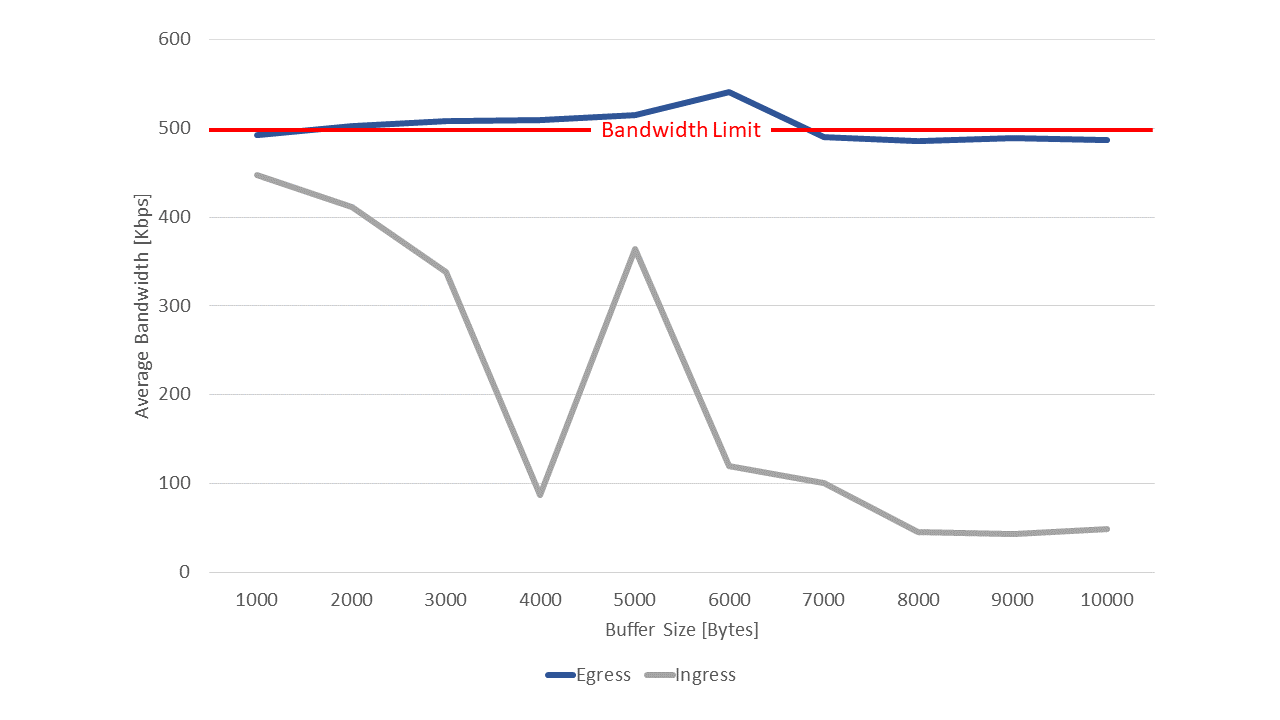
\includegraphics[width=\textwidth]{img/Evaluation-Bandwidth-Wondershaper.png}
	\caption{Evaluation of the Bandwidth (Wondershaper)}
	\label{Evaluation of the Bandwidth (Wondershaper)}
\end{figure}

\begin{figure}[h]
	\centering
	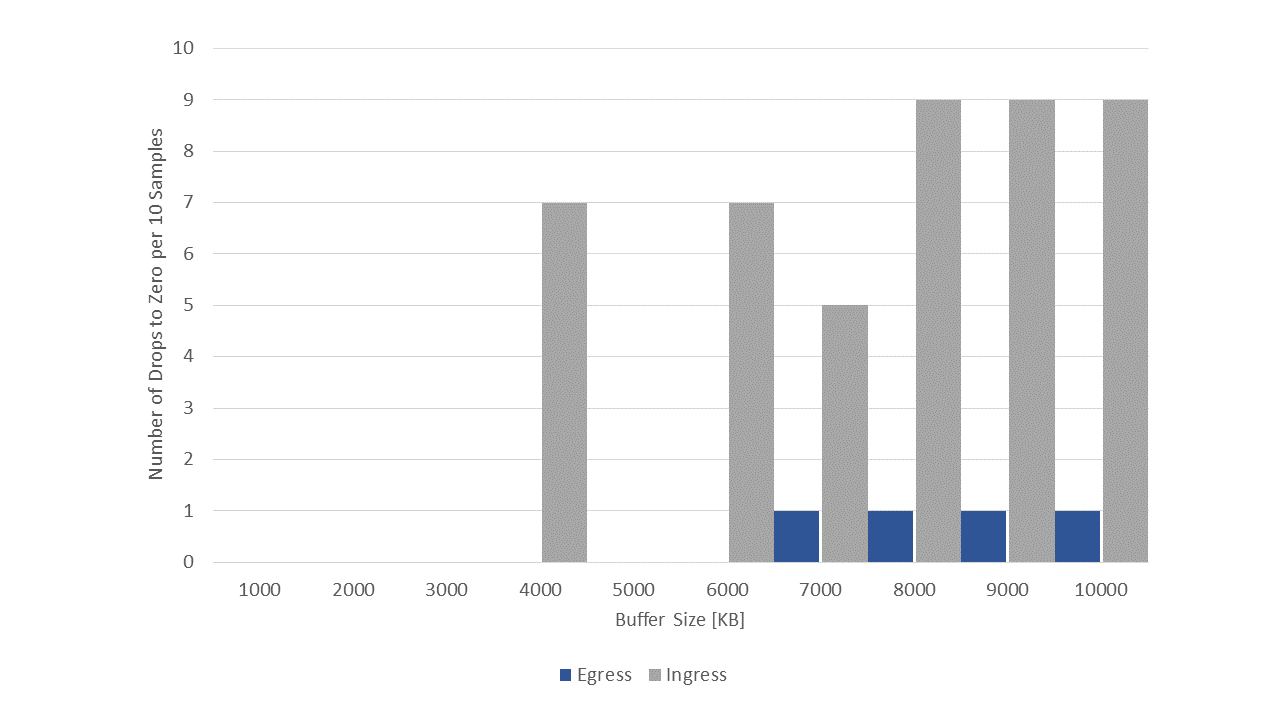
\includegraphics[width=\textwidth]{img/Evaluation-Zeros-Wondershaper.png}
	\caption{Evaluation of Bandwidth Drops (Wondershaper)}
	\label{Evaluation of the Bandwidth Drops (Wondershaper)}
\end{figure}

\newpage
\subsection{Examination of the Problem with Ingress Traffic}

\chapter{Conclusion}
\section{Front End}

Implementing the front end was the easiest part of the entire project. For that, I stuck mostly to the current practices and implemented the mechanisms that were additionally used for this project in a manner that is very similar to the mechanisms that were already in place. The intention of this approach was to make maintainability as easy as possible, especially since the \acs{SCIONLab} server is still in development. I also made sure that the code that I contributed was well documented and easy to read.

\section{Back End}

Designing and implementing the \textit{scionlab\_bw\_limiter} was definitely the part of the project that required the most research. Understanding and configuring \acs{TC} turned out to be harder than expected. Furthermore it is quite unfortunate that there isn't really a reasonable \acs{API} that let's us configure \acs{TC} using Python. Therefore I had to write my own wrapper for \acs{TC}. But I think that the implementation of the \textit{scionlab\_bw\_limiter} works quite well and is also easy to understand. The results the \textit{scionlab\_bw\_limiter} delivers are not perfect, but still satisfiable, especially since there is not really a tool out there (of which I know) that performs better. Especially the results for ingress traffic were not as good as I hoped they would be. But there it is also questionable on whether the measurements of iPerf3 were accurate or not. At least I showed that the quite established bandwidth limiter \textit{wondershaper} behaves similarly.

\section{Difficulties that Arouse}

The biggest challenge I was facing, was enforcing a bandwidth limit on ingress traffic. \acs{TC} was mainly designed to do traffic shaping in order to improve the quality of service. For improving the quality of service, egress traffic is much more relevant than ingress traffic. Therefore \acs{TC} is not as advanced when it comes to handling ingress traffic as I wished it would be.
\\
Furthermore, testing turned out to be quite difficult as well. It's not easy to create a realistic test environment, which is still simple enough such that test results can be interpreted in a meaningful way. If test results turn out differently than expected, it is often not clear whether the measurement was wrong, the test configuration was faulty, the test environment was unrealistic or the implementation was buggy. It might as well just be that the testing tool is limited in it's measurement capabilities. 

\section{Lessons Learned}

This bachelor thesis project offered me the opportunity to gain a deep understanding of how \acs{IP} traffic can be managed in order to enforce a bandwidth limit and what possible complications and consequences there can be. It also provided me with a holistic view over \acs{SCION}, \acs{SCIONLab} and in general how a novel internet architecture can be tested in a distributed testbed. It also gave me a better understanding of how Linux tools work that are used for networking purposes. Last but not least, it again showed me the importance of extensive testing and how hard it is to have an accurate and easy to use testing tool.


\appendix

\chapter{Abbreviations}
\begin{acronym}[SCIONLab]%longest acronym in [] to align
	\acro{AP}{Attachment Point}
	\acro{AS}{Autonomous System}
	\acrodefplural{AS}[ASes]{Autonomous Systems}
	\acro{AWS}{Amazon Web Services}
	\acrodefplural{AWS}[AWS]{Amazon Web Services}
	\acro{BGP}{Border Gateway Protocol}
	\acro{BR}{Border Router}
	\acro{BS}{Beacon Server}	
	\acro{CS}{Certificate Server}
	\acro{ETH}{Eidgenössische Technische Hochschule (Swiss Federal Institute of Technology)}
	\acro{HTB}{Hierarchy Token Bucket}
	\acro{IP}{Internet Protocol}
	\acro{ISD}{Isolation Domain}
	\acro{ISP}{Internet Service Provider}
	\acro{JSON}{JavaScript Object Notation}
	\acro{OSI}{Open Systems Interconnection}
	\acro{PCB}{Path-Segment Construction Beacon}
	\acro{PS}{Path Server}
	\acro{QDISC}{Queuing Discipline}
	\acro{SCION}{Scalability, Control and Isolation on Next-Generation Networks}
	\acro{SCIONLab}{Testbed for SCION}
	\acro{TBF}{Token Bucket Filter}
	\acro{TC}{Traffic Control}
	\acro{TRC}{Trust Root Configuration}
	\acro{VM}{Virtual Machine}
\end{acronym}



\backmatter

\printbibliography
%\bibliographystyle{plain}
%\bibliography{refs}

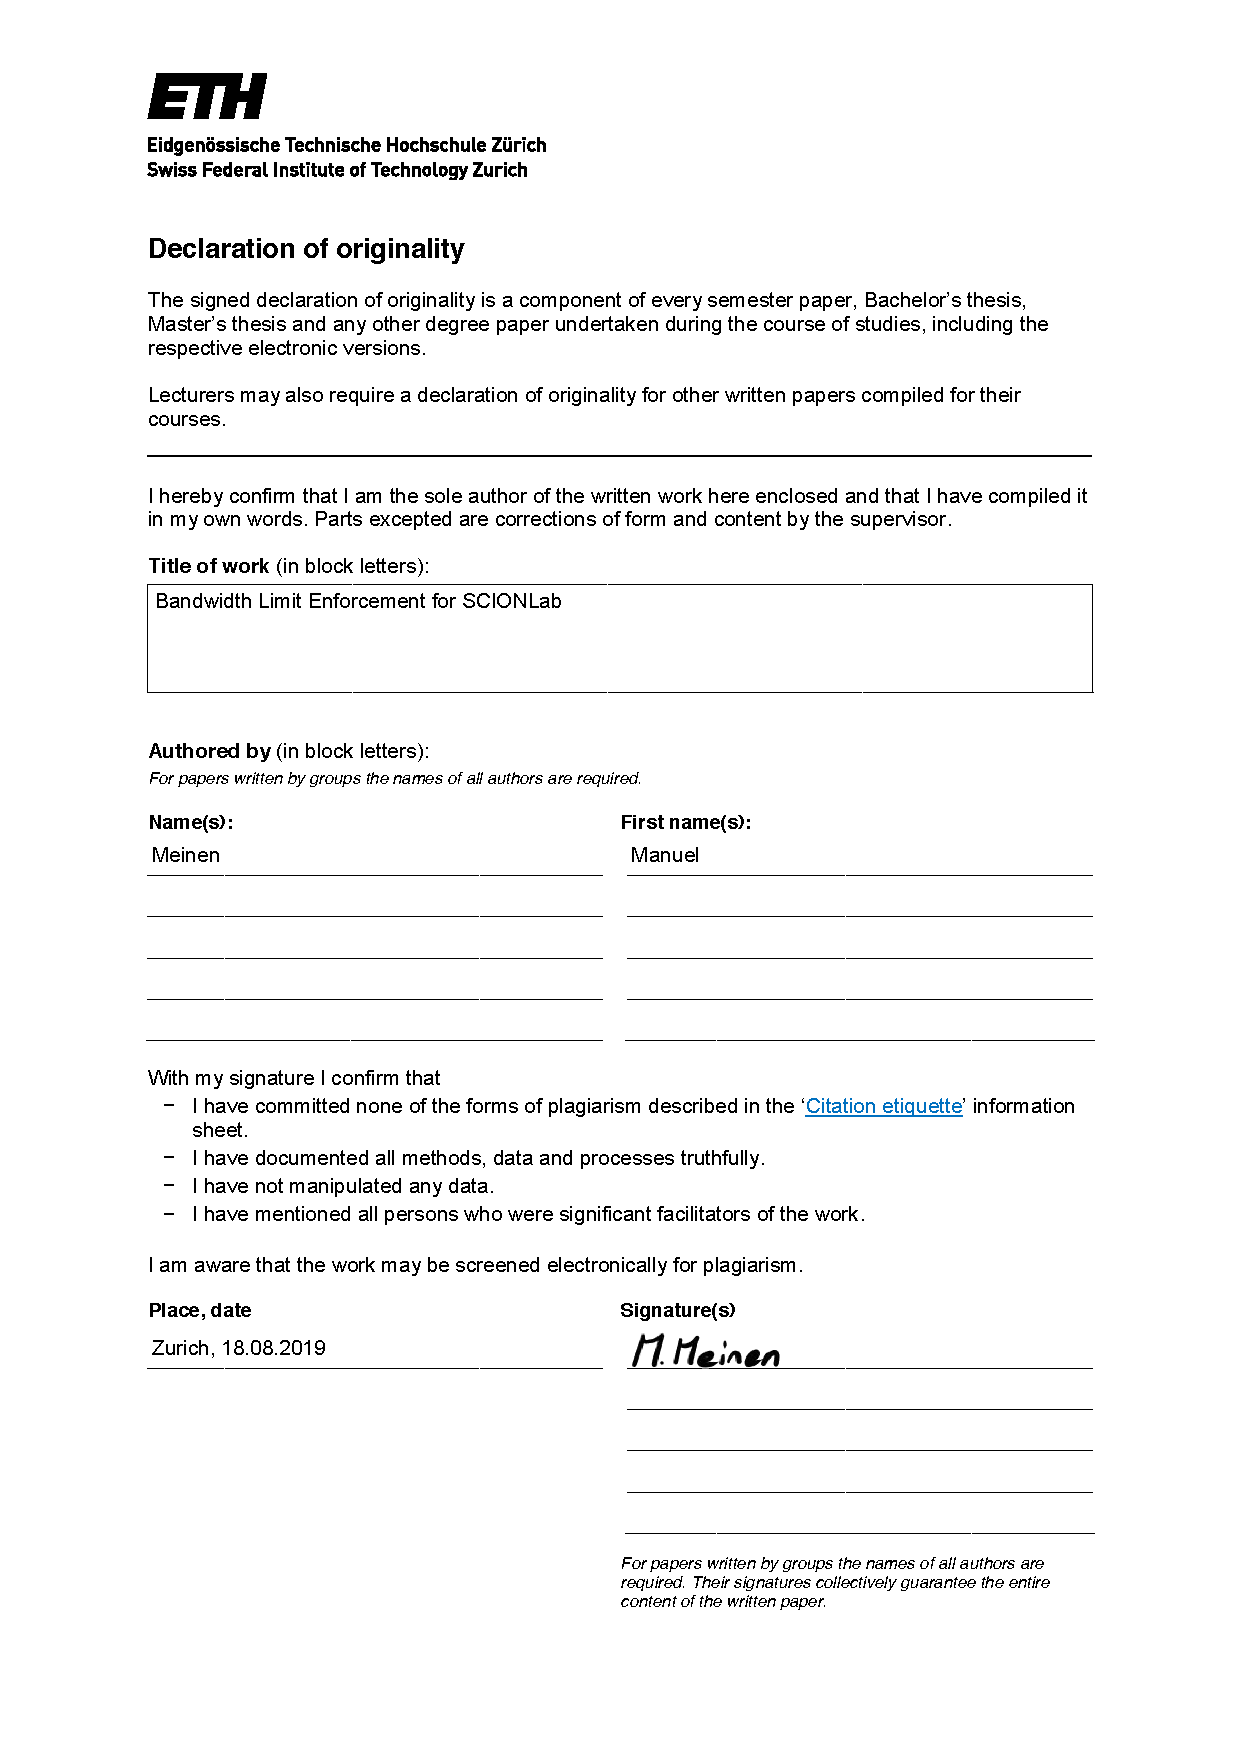
\includepdf[pages={-}]{declaration-originality.pdf}

\end{document}
